\documentclass[12pt]{article}

\usepackage{sbc-template}
\usepackage[english]{babel}
\usepackage[utf8]{inputenc}
\usepackage[table]{xcolor}
\usepackage{booktabs}
\usepackage[colorinlistoftodos,prependcaption,textsize=footnotesize]{todonotes}

\graphicspath{{./img/}}

\setcounter{secnumdepth}{2}
\setcounter{tocdepth}{2}

\title{A New Program Autotuning Methodology Using Cloud Computing and OpenTuner}
\author{Pedro Bruel, Alfredo Goldman, Daniel Batista}
\address{Instituto de Matemática e Estatística (IME)\\
Universidade de São Paulo (USP)\\
R. do Matão, 1010 – Cidade Universitária, São Paulo – SP, 05508-090\\
\email{\{phrb,gold,batista\}@ime.usp.br}
}

\begin{document}

\maketitle

\begin{abstract}

%This sequential search takes even longer to find
%optimizations for programs with considerable execution times. 

%Although an autotuner is able to find incrementally better solutions
%quickly, finding good configurations typically takes a very long time.

The OpenTuner framework provides domain-agnostic tools for the implementation of autotuners. It sequentially evaluates program configurations exploring search spaces that are commonly very large. This paper proposes a new methodology and a protocol for the distributed execution of autotuners. Both contributions are implemented in the OpenTuner framework as an extension to the OpenTuner measurement driver by distributing and parallelizing the measurement process via cloud computing resources. The performance evaluation shows that autotuners implemented with the extension are able to achieve good performance using few and cheap cloud computing resources, lowering the cost and the power consumption of producing an autotuned solution.

    \todo[inline,author=Pedro]{A very short summary of the results will be
    provided in the abstract, as well as a brief discussion of the
    result normalization research question.}
\end{abstract}

\section{Introduction} \label{sec:intro}

\todo[inline,author=Disclaimer]{This is a draft of the paper. The results and
implementations are not final or completed. Future versions will improve
the presentation and present results and conclusions. The maximum page count
for SBRC is 14 pages, and this document is 12 pages long.}

The program autotuning problem fits in the framework of the Algorithm Selection
Problem, introduced by Rice in 1976~\cite{rice1976algorithm}. The objective of
an autotuner is to select the best algorithm, or algorithm configuration, for
each instance of a problem.  Algorithms or configurations are selected
according to performance metrics such as the time to solve the problem
instance, the accuracy of the solution and the energy consumed.  The set of all
possible algorithms and configurations that solve a problem defines a
\emph{search space}. Various optimization techniques search this space, guided
by the performance metrics, for the algorithm or configuration that best solve
the problem.

Autotuners can specialize in domains such as matrix
multiplication~\cite{bilmes1997phipac}, dense~\cite{whaley1998atlas} or
sparse~\cite{vuduc2005oski} matrix linear algebra, and parallel
programming~\cite{jordan2012multi}. Other autotuning frameworks provide more
general tools for the representation and search of program configurations,
enabling the implementation of autotuners for different problem
domains~\cite{ansel2014opentuner,hutter2009paramils}.

The OpenTuner framework~\cite{ansel2014opentuner} provides tools for the
implementation of autotuners for various problem domains. It implements
different search techniques that explore the same search space for program
optimizations. Although support for parallel compilation is provided in the
framework the empirical exploration of the search space, that is, running and
measuring program execution time, is done sequentially.

The main contribution of this paper is the implementation of an
OpenTuner extension that distributes and parallelizes the exploration of
the optimization space by combining results obtained from virtual machines
in a cloud computing environment. A local machine (LM) runs the main
OpenTuner application and several virtual machines (VM) run measurement
modules that provide results when requested, performing a more efficient
exploration of the search space.

The interactions between the local and virtual machines follows
the client-server model. The local machine runs a measurement client that
requests results from various measurement servers running in virtual machines
hosted at the Google Compute Engine (GCE).
We compare the performance of our extension with the
unmodified framework in a diverse benchmark of applications, identifying
the problem domains that benefit from this cloud-based approach.

The rest of the paper is organized as follows.
Section~\ref{sec:related} discusses related work.
Section~\ref{sec:ot} discusses the architecture of the OpenTuner framework.
Section~\ref{sec:ext} presents the architecture of the measurement driver
extension, the GCE interface and the application protocol
that mediates the interactions between the \emph{MeasurementClient} and
\emph{MeasurementServer}s.
Section~\ref{sec:norm} discusses the result normalization strategies.
Section~\ref{sec:exp} describes the experiments performed and the
applications used in the benchmark.
Section~\ref{sec:results} discusses the results.
Section~\ref{sec:conclusion} concludes.

\section{Related Work} \label{sec:related}

Rice's conceptual framework~\cite{rice1976algorithm} formed the foundation
of autotuners in various problem domains.  In 1997, the PHiPAC
system~\cite{bilmes1997phipac} used code generators and search scripts to
automatically generate high performance code
for matrix multiplication. Since then, systems tackled different domains with a
diversity of strategies. Whaley \emph{et al.}~\cite{whaley1998atlas} introduced
the ATLAS project, that optimizes dense matrix multiply routines. The
OSKI~\cite{vuduc2005oski} library provides automatically tuned kernels for
sparse matrices. The FFTW~\cite{frigo1998fftw} library provides tuned C
subroutines for computing the Discrete Fourier Transform.  In an effort to
provide a common representation of multiple parallel programming models, the
INSIEME compiler project~\cite{jordan2012multi} implements abstractions for
OpenMP, MPI and OpenCL, and generates optimized parallel code for heterogeneous
multi-core architectures.

Some autotuning systems provide generic tools that enable the implementation of
autotuners in various domains. PetaBricks~\cite{ansel2009petabricks} is a
language, compiler and autotuner that introduces abstractions, such as the
\texttt{\footnotesize either...or} construct, that enable programmers to define
multiple algorithms for the same problem.  The ParamILS
framework~\cite{hutter2009paramils} applies stochastic local search methods
for algorithm configuration and parameter tuning.  The OpenTuner
framework~\cite{ansel2014opentuner} provides ensembles of techniques that
search spaces of program configurations. Bosboom \emph{et al.} and Eliahu use
OpenTuner to implement a domain specific language for data-flow
programming~\cite{bosboom2014streamjit} and a framework for recursive parallel
algorithm optimization~\cite{eliahu2015frpa}.

In a progression of papers~\cite{gupta2012exploring,gupta2014evaluating,gupta2013hpccloud},
Gupta \emph{et al.} provide experimental evaluations of the application of
cloud computing to high performance computing, describing which kind of
applications has the greatest potential to benefit from cloud computing.
Their work highlights small and medium scale projects as the main beneficiaries
of cloud computing resources.

\todo[inline,author=Pedro]{Provide a better discussion of Gupta et al.'s
results.}
\todo[inline,author=Pedro]{Justify the choice of OpenTuner as the modified
system, by saying it is a domain-agnostic tool that has, to the best of our
knowledge, no equivalent in scope.}

\section{OpenTuner} \label{sec:ot}

OpenTuner search spaces are defined by \emph{Configuration}s, that are composed
of \emph{Parameter}s of various types. Each type has restricted bounds and
manipulation functions that enable the exploration of the search space.
OpenTuner implements ensembles of optimization techniques that
perform well in different problem domains. The framework uses
\emph{meta-techniques} to coordinate the distribution of resources
between techniques.
Results found during search are shared through a
database. An OpenTuner application can implement its own search
techniques and meta-techniques, making the ensemble more robust.
The source code is available\footnote{Hosted at GitHub:
\texttt{\scriptsize github.com/jansel/opentuner}} under the MIT License.

\begin{figure}[htpb]
    \centering
    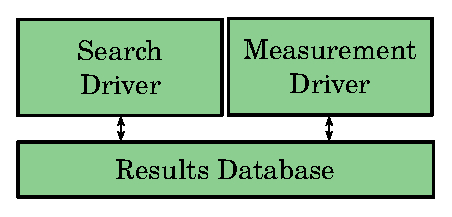
\includegraphics[scale=.62]{opentuner-implementation}
    \caption{Simplified OpenTuner Architecture.}
    \label{fig:ot-imp}
\end{figure}

Figure~\ref{fig:ot-imp} shows a high-level view of OpenTuner's architecture.
Measurement and searching are done in separate modules, whose main classes are
called \emph{drivers}. The search driver requests measurements by registering
configurations to the database. The measurement driver reads those
configurations and writes back the desired results.  Currently, the
measurements are performed sequentially.

OpenTuner implements optimization techniques such as the
Nelder-Mead~\cite{nelder1965simplex} simplex method and Simulated
Annealing~\cite{kirkpatrick1983optimization}. A resource sharing mechanism,
called \emph{meta-technique}, aims to take advantage of the strengths of each
technique by balancing the exploitation of a technique that has produced good
results in the past and the exploration of unused and possibly better ones.

\todo[inline,author=Pedro]{Compare sequential and parallel tuning. Describe
when OpenTuner uses threads to compile target programs.}

\section{Implementation Details}
\label{sec:ext}

The implementation follows the client-server model, distributing
measurements of program configurations between a group of virtual
machines running \emph{MeasurementServer}s in the GCE. The servers
waits for measurement requests from a client, and maintain copies
of the program to be autotuned and the user-defined function that
measures configurations.

An interface was also implemented to encapsulate the communication
from the client enabling a considerably lower implementation
effort for the client. Figure~\ref{fig:loc-comp} show a rough
estimate of the implementation effort for the three components
of the implementation.

The machine running the OpenTuner autotuner runs a \emph{MeasurementClient},
an extension of the native \emph{MeasurementDriver}, that instead of
compiling and running result requests locally, uses the GCE interface to
route requests to virtual machines and them saves the results to the local
database.

\begin{figure}[htpb]
    \centering
    \begin{minipage}{.45\textwidth}
        \centering
        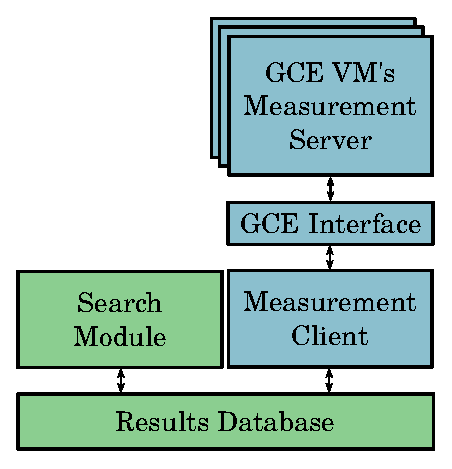
\includegraphics[scale=.64]{high-level-implementation}
        \caption{A high-level view of the architecture.}
        \label{fig:high-level}
    \end{minipage}%
    \hfill
    \begin{minipage}{.45\textwidth}
        \centering
        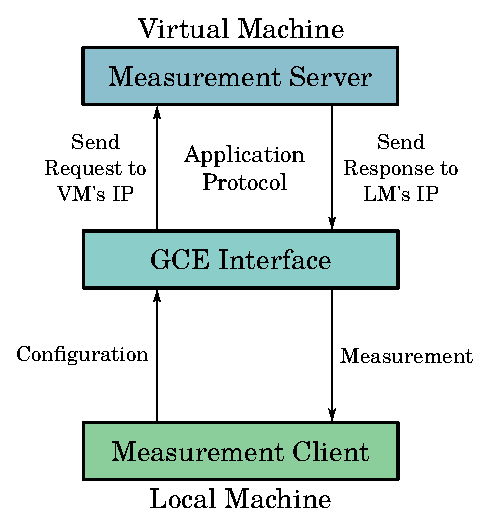
\includegraphics[scale=.64]{low-level-implementation}
        \caption{A lower-level view of the architecture.}
        \label{fig:low-level}
    \end{minipage}%
    \label{fig:archs}
\end{figure}

Figures~\ref{fig:high-level} and~\ref{fig:low-level} present an
overview of the architecture of the extension.
Figure~\ref{fig:high-level} presents the architecture of an OpenTuner
application running the measurement client and communicating with the
measurement servers.  Green boxes in the figure represent OpenTuner modules
that will not be modified, and blue boxes represent new or modified modules.

Figure~\ref{fig:low-level} shows, on a lower level of abstraction, the
interactions between the measurement client and servers. The client
requests results from the server through a wrapper of the GCE Python API.
The GCE interface also encapsulates the application protocol used in
the client-server communication.

The remaining of this section describes the extension implementation in further
detail, the GCE interface and the application protocol.

\begin{figure}[htpb]
    \centering
    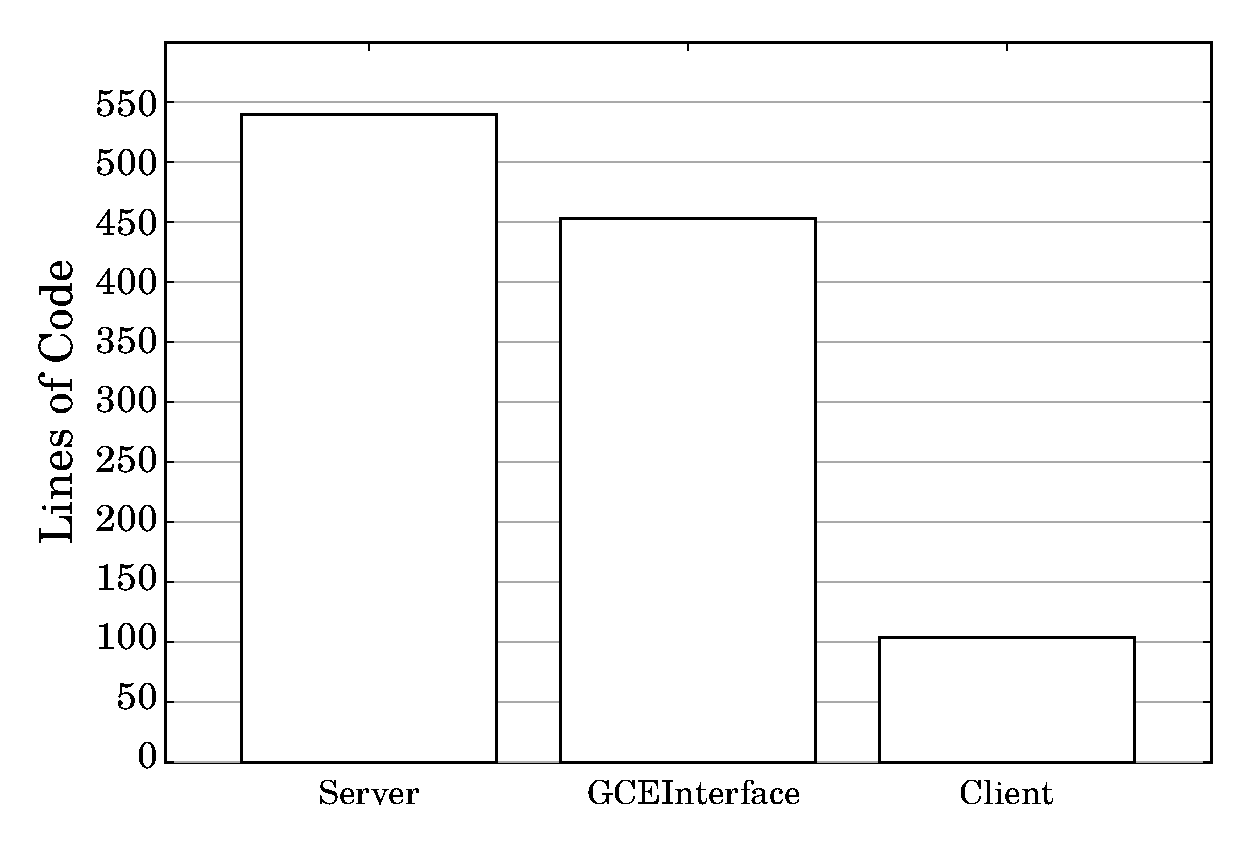
\includegraphics[scale=.35]{loc_comparison}
    \caption{An estimate of the implementation effort, measured in lines of code.}
    \label{fig:loc-comp}
\end{figure}

\subsection{Measurement Server and Client}
\label{sec:server-client}

OpenTuner controls the execution flow of an application with the
\texttt{\footnotesize main} function of the \emph{TuningRunMain} class. This
function initialises the database and the search and measurement modules. It
then calls the \texttt{\footnotesize main} function of the search driver, which
runs the main loop of the application.  The search driver generates
configurations to be tested and saves them to the database. It then calls the
\texttt{\footnotesize process\_all} function of the measurement driver and
blocks until the function returns.

The \texttt{\footnotesize process\_all} function calls the
\texttt{\footnotesize run\_desired\_results} function, which is able to run
compilations in parallel but only sequential measurements.  The modified
\emph{MeasurementDriver} initialises the GCE interface during its own
initialisation. During execution the overridden \texttt{\footnotesize
process\_all} and \texttt{\footnotesize run\_desired\_results} functions route
the result requests to the virtual machines using the \emph{GCEInterface}.

An instance of the \emph{MeasurementServer} runs in every virtual machine. The
server is installed after the machine's initialisation and waits for TCP
connections from a single client. The application protocol used in
communications between the clients and servers is described in
Section~\ref{sec:app}.

\subsection{GCE Interface}
\label{sec:gce}

The interactions between the local \emph{MeasurementClient} and the virtual
machines' \emph{MeasurementServer}s are mediated by the
\emph{GCEInterface}, a wrapper of the GCE Python API.
The interface starts and configures virtual machines
storing each measurement server's IP.

The interface enables the \emph{MeasurementClient} to request results from
the servers without knowledge of the application protocol. Running our
client-server implementation in another cloud environment would require a
new interface that manages virtual machines in this environment, but no
modifications are needed to the server or client.

\subsection{Application Protocol}
\label{sec:app}

This section describes the text-based application protocol used in the
client-server communications mediated by the \emph{GCEInterface}. Note the
\texttt{\footnotesize CLONE} message. The user's OpenTuner application must
be a git project available via \texttt{\footnotesize{HTTP}}. The application
will be cloned to the virtual machine by the server and used to obtain the
autotuning results requested by the client.

\paragraph{Messages}
\newcolumntype{K}{>{\centering\arraybackslash}m{5cm}}
\newcommand{\specialcell}[2][c]{%
  \begin{tabular}[#1]{@{}K@{}}#2\end{tabular}}

\newcolumntype{T}{>{\centering\arraybackslash}m{1.5cm}}
\newcolumntype{L}{>{\centering\arraybackslash}m{2.4cm}}

\begin{table}[htpb]
    \centering
    \tiny
    \begin{tabular}{@{}TLK@{}}
        \toprule
        {\bf Command} & {\bf Function} & {\bf Message} \\ \midrule
        {\tiny \bf START} & 
        {\tiny Sets the server's status to AVAILABLE} & 
        {\tiny \tt ``START''} \\ \midrule
        {\tiny \bf STOP} & 
        {\tiny Sets the server's status to STOPPED} & 
        {\tiny \tt ``STOP''} \\ \midrule
        {\tiny \bf STATUS} & 
        {\tiny Requests the server current status} & 
        {\tiny \tt ``STATUS''} \\ \midrule
        {\tiny \bf DISCONNECT} & 
        {\tiny Disconnects from the server} & 
        {\tiny \tt ``DISCONNECT''} \\ \midrule
        {\tiny \bf SHUTDOWN} & 
        {\tiny Disconnects and shuts the server down} & 
        {\tiny \tt ``SHUTDOWN''} \\ \midrule
        {\tiny \bf CLONE} & 
        {\tiny Clones a git repository to the virtual machine} & 
        {\tiny \tt ``CLONE REPO\_URL DIST\_DIR''} \\ \midrule
        {\tiny \bf LOAD} & 
        {\tiny Imports the user's MeasurementInterface into the server} & 
        {\tiny \tt ``LOAD TUNER\_PATH INTERFACE\_NAME''} \\ \midrule
        {\tiny \bf MEASURE} & 
        {\tiny Computes the measurement for a given configuration} & 
        {\tiny \tt ``MEASURE CONFIG INPUT LIMIT''} \\ \midrule
        {\tiny \bf GET} & 
        {\tiny Requests a configuration's result} & 
        {\tiny \tt ``GET RESULT\_ID''} \\ \bottomrule
    \end{tabular}
    \caption{Server messages.}
    \label{tab:protocol-messages}
\end{table}


Table~\ref{tab:protocol-messages} shows all the messages in the protocol,
a brief description of their meaning and their string format. The client
must send a \texttt{\footnotesize MEASURE} message for each configuration
that is measured. The server returns a unique ID that is used to retrieve
the results when they are ready. This is done by sending a
\texttt{\footnotesize GET} message.

\paragraph{Server Responses}

The server responds to each request with a message template and
trailing, message-specific parameters. Responses always start
with the correspondent command name and end with a newline character.
Each response contains the current server status (\texttt{\footnotesize SERVER\_STATUS})
and error code of the command (\texttt{\footnotesize ERROR\_STATUS}).
The optional argument list (\texttt{\footnotesize [ARGS..]}) contains the
measurement result, for example, in the case of a successful
\texttt{\footnotesize GET} response. Figure~\ref{fig:response-template}
shows the format of a server response.

\begin{figure}[htpb]
    \centering
    \footnotesize
    \begin{tabular}{@{}c@{}}
        \toprule
        {\tt \lq{}COMMAND ERROR\_STATUS SERVER\_STATUS [ARGS..] [MESSAGE]\rq{}} \\ \bottomrule
    \end{tabular}
    \caption{The format of a server response.}
    \label{fig:response-template}
\end{figure}

\paragraph{Code Availability}

The code for the measurement server, client and the interface is
available\footnote{All code is hosted at GitHub: \\ \texttt{\scriptsize
github.com/phrb/measurement-server} \\ \texttt{\scriptsize
github.com/phrb/gce\_interface} \\ \texttt{\scriptsize
github.com/phrb/measurement\_client}} under the GNU General Public License.

\section{Result Normalization}
\label{sec:norm}

\todo[inline,author=Pedro]{This discussion will probably be left out
of this version of the paper, since we did not run experiments with
architecture-dependant problems.}

Using a cloud environment, an autotuner will typically optimize programs for
a machine with a different architecture from the virtual machines. A
normalization technique must be devised that enables the results found in the
virtual machines to be valid for the local machine.  We present four
approaches to this problem. The best approach for each problem domain
must be experimentally determined, and could be a combination of the approaches
described here.

\paragraph{Autotune Performance Models}
Another autotuner could be implemented to optimize parameters of a simple
performance model, that would associate a configuration's measurement and the
virtual machine that produced it with a conversion function that transposes
performance results to the target architecture.

\paragraph{Ensembles of Virtual Machines}
The cloud application could be composed of virtual machines with different
architectures. The final performance measurement for a configuration would be
built from some combination of the results obtained in these different virtual
machines.

\paragraph{Architecture Simulators}
The target machine could be modeled by an architecture simulator such as
\emph{zsim}~\cite{sanchez2013zsim}, a simulator for multi-core architectures
available\footnote{Hosted at GitHub: \texttt{\scriptsize
https://github.com/s5z/zsim}} under the GNU General Public License.  Using a
simulator would solve the normalization problem but introduce other problems,
such as the simulator's accuracy and performance.

\paragraph{Autotune in the Cloud}
Finally, the normalization problem could be sidestepped, at least in initial
stages of research, by running the servers and clients in the cloud using
the same kind of virtual machine.

\section{Experiments} \label{sec:exp}

This section describes the problems that compose the benchmark and the Google
Compute Engine's virtual machines and project settings.  The performances of
the autotuners for each problem in the benchmark were measured in 12 different
experimental settings. Each tuning run lasted 15 minutes, used 2, 4 or 8
virtual machines, and was repeated 4 times.  We also varied the number of
result requests that each virtual machine in a tuning run processed, namely 1,
4, 8 or 16 requests per machine.

\subsection{Using the Google Compute Engine}

All virtual machines used in the experiments had a single vCPU and 3.75Gb of
RAM (Google Compute Engine machine type \texttt{\footnotesize n1-standard-1}).
All experiments were performed with machines from the \texttt{\footnotesize
us-central1-f} zone. We built a virtual machine image with the latest stable
Debian distribution and all dependencies installed, speeding up the virtual
machines' initialization time.

\subsection{Travelling Salesperson Problem}

The instances of the Travelling Salesperson Problem (TSP) used in the
experiments in this paper were obtained from TSPLIB~\cite{reinelt1991tsplib}.
A TSP solver was implemented as an OpenTuner application. The search space was
defined by all the possible permutations, or tours, of cities where the first
and last cities are the same. We used two instances, of size 532 and 85900.

\section{Results} \label{sec:results}

\todo[inline,author=Pedro]{This section will present and discuss the results,
connecting the findings with normalization techniques and problem domains.}

\subsection{Travelling Salesperson Problem}

\todo[inline,author=Pedro]{Here we will discuss the results for the TSP. We
will argue that we achieved results very close to a high-end machine
using cheap and low-end virtual machines.}

\begin{figure}[htpb]
    \centering
    \begin{minipage}{.45\textwidth}
        \centering
        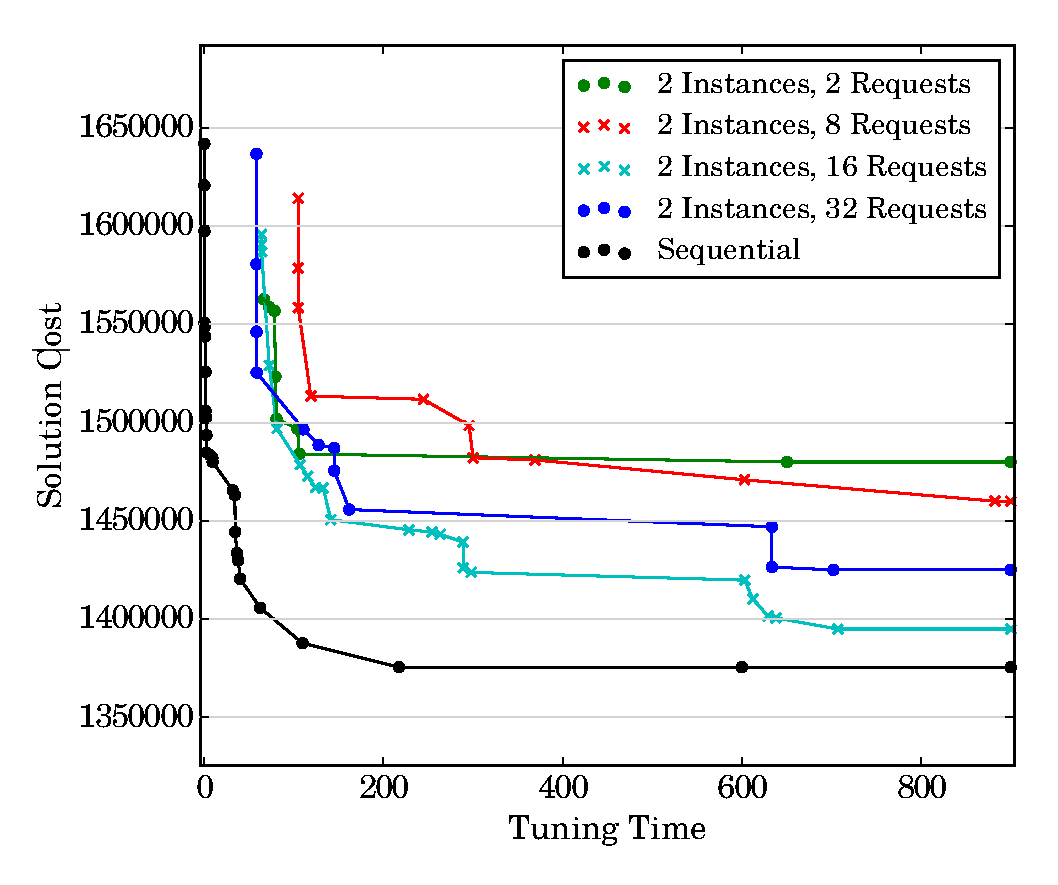
\includegraphics[scale=.35]{i2_p_n_comparison}
        \caption{Measurements using two virtual machine instances, solving
                 a TSP instance of size 532.}
        \label{fig:high-level}
    \end{minipage}%
    \hfill
    \begin{minipage}{.45\textwidth}
        \centering
        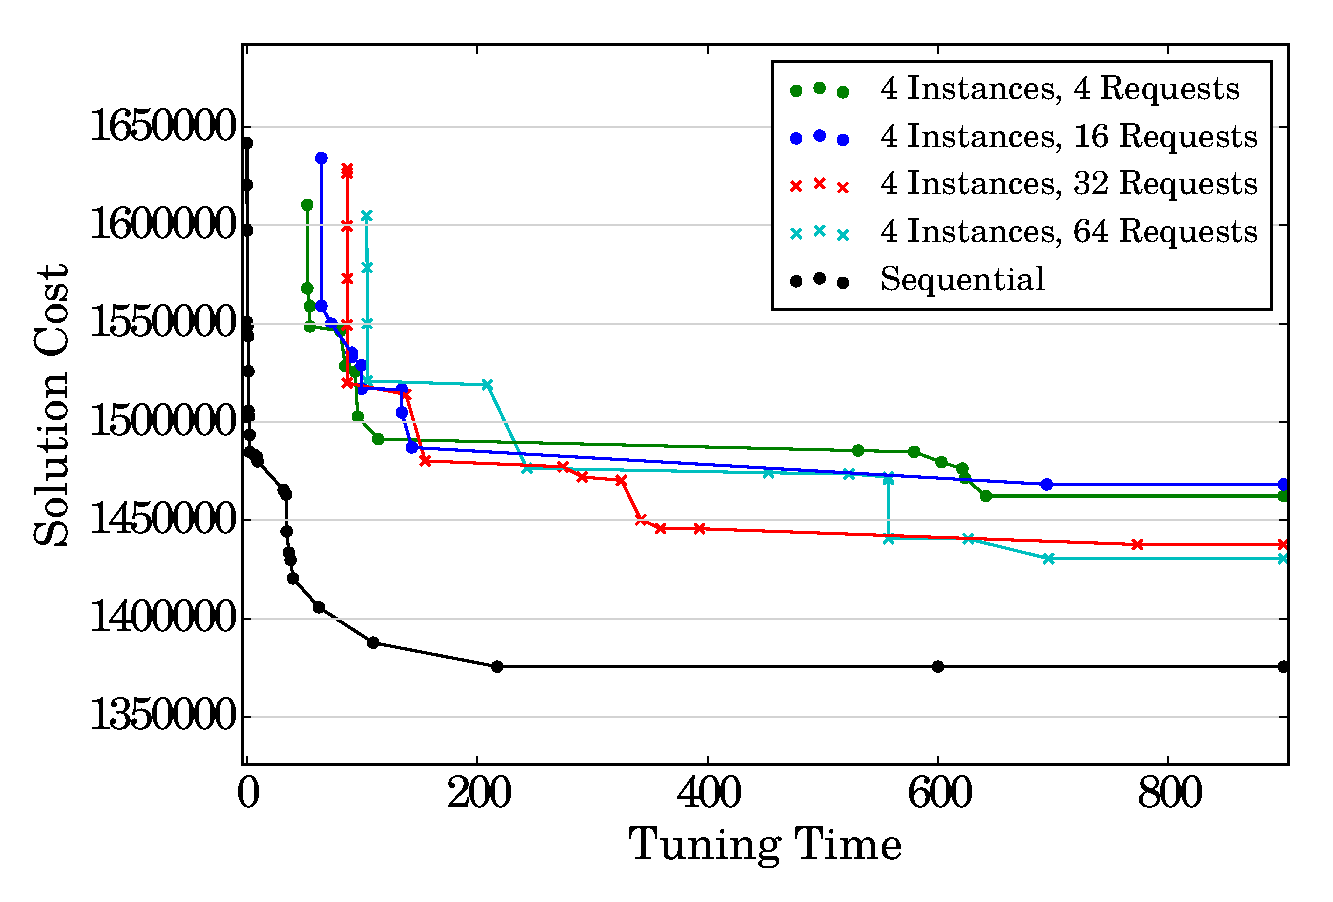
\includegraphics[scale=.35]{i4_p_n_comparison}
        \caption{Measurements using four virtual machine instances,
                 solving a TSP instance of size 532.}
        \label{fig:low-level}
    \end{minipage}%
    \label{fig:archs}
\end{figure}

\begin{figure}[htpb]
    \centering
    \begin{minipage}{.45\textwidth}
        \centering
        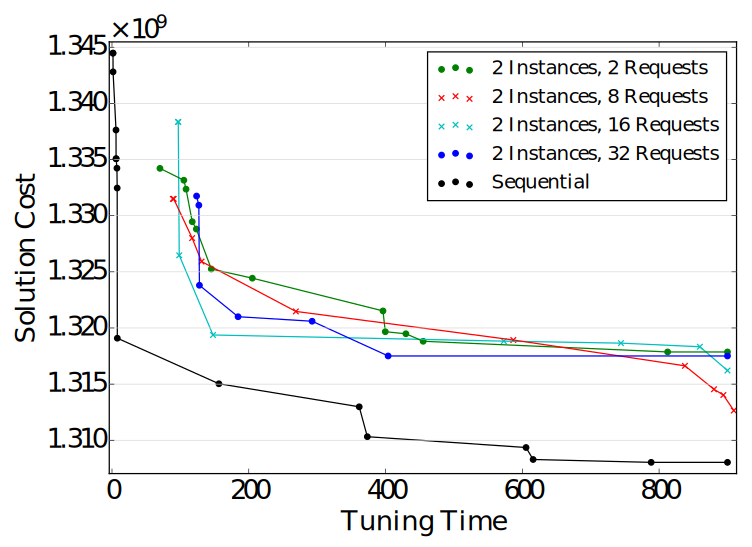
\includegraphics[scale=.35]{i2_p_n_comparison_85900}
        \caption{Measurements using two virtual machine instances,
                 solving an instance of size 85900.}
        \label{fig:high-level}
    \end{minipage}%
    \hfill
    \begin{minipage}{.45\textwidth}
        \centering
        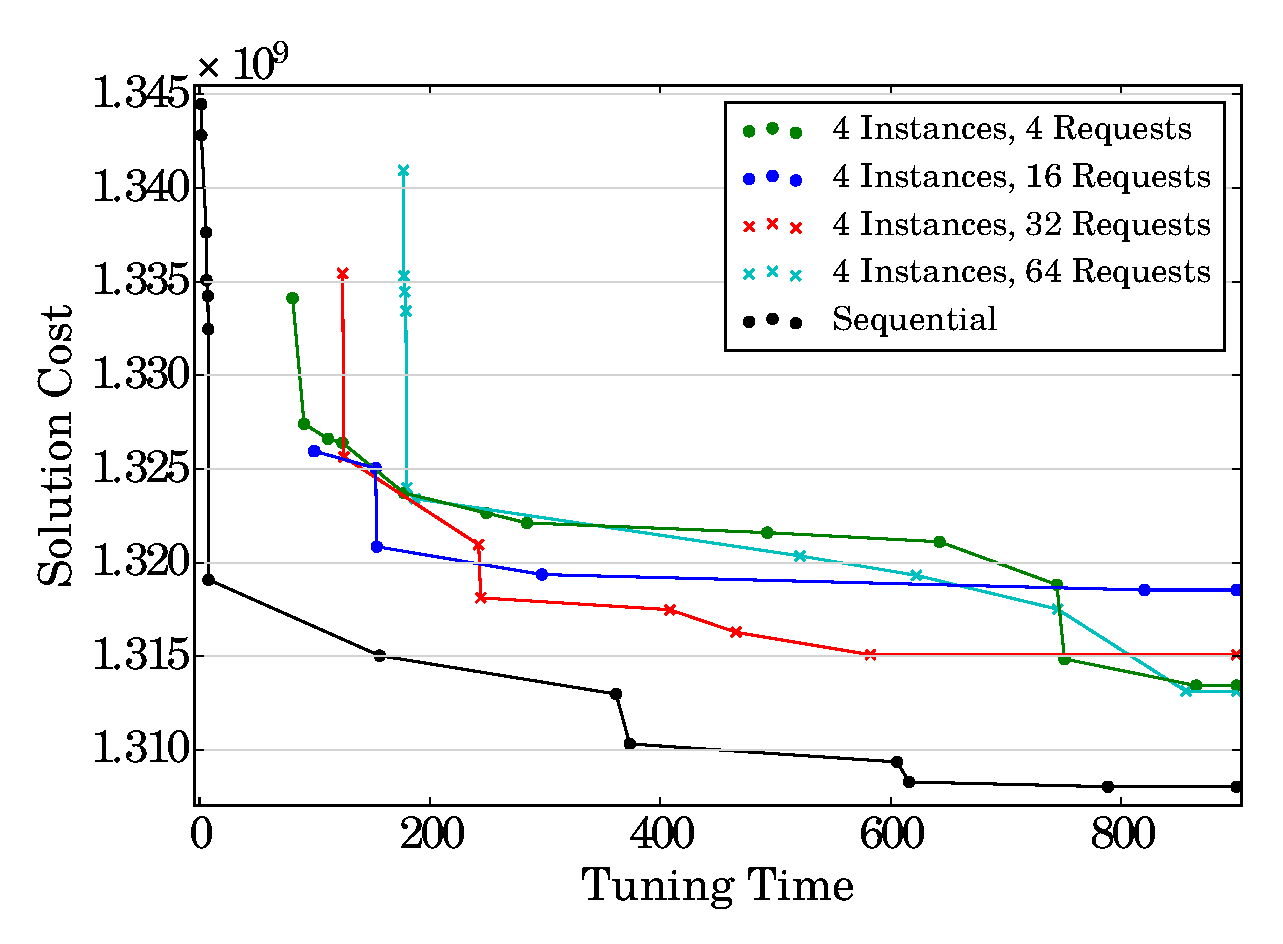
\includegraphics[scale=.35]{i4_p_n_comparison_85900}
        \caption{Measurements using four virtual machine instances,
                 solving an instance of size 85900.}
        \label{fig:low-level}
    \end{minipage}%
    \label{fig:archs}
\end{figure}

\section{Conclusion} \label{sec:conclusion}

This paper presented an extension of the OpenTuner autotuning framework
enabling it to leverage the cloud computing resources from GCE.  We propose
four approaches to solve the result normalization problem which would enable
transposing the results obtained in virtual machines to a local machine.

\bibliographystyle{IEEEtran}
\bibliography{IEEEabrv,ref}

\end{document}
